\documentclass[20pt, a0paper, landscape, colspace=9mm, subcolspace=4mm, blockverticalspace=9mm, innermargin=8mm, margin=0mm]{tikzposter}
\title{\parbox{\linewidth}{\centering Bayesian Non-Parametric Inference
                        in Multivariate\\ Peaks-over-Thresholds Models}}
\author{Peter Trubey \& Bruno Sans{\'o}}
\date{September 7, 2022}
\institute{UC Santa Cruz; Department of Statistics}

\usepackage[english]{babel}
\usepackage{blindtext}
\usepackage{amsmath}
\usepackage{amssymb}
\usepackage{bm}
\usepackage{comment}
\usepackage{nccmath}
\usepackage{booktabs}
\usepackage{enumitem}
\usepackage{graphicx}
\usepackage{wrapfig}
\usepackage{adjustbox}

\usetheme{Simple}

\begin{document}

\maketitle

\begin{columns}
    \column{0.333}
    \block{Multivariate Peaks-over-Thresholds}{
        For $d$-dimensional random vector $\bm{W} = (W_1,\ldots,W_d) \sim F$;   
        assume the existence of sequences of vectors $\bm{a}_n,\bm{b}_n$ such that 
        \[\lim\limits_{n\to\infty}F^n\left(\bm{a}_n\bm{w} + \bm{b}_n\right) = G(\bm{w}),\] 
        then $G$ is a $d$-variate GEV.  It follows that\\
        \[
        \lim\limits_{n\to\infty}\text{Pr}\left(\frac{\bm{W} - \bm{b}_n}{\bm{a}_n} \leq \bm{w}\mid \bm{W} 
            \not\leq \bm{b}_n\right) = \frac{\log G(\bm{w}\wedge \bm{0}) - \log G(\bm{w})}{\log G(\bm{0})} = H(\bm{w}),
            \]\\
        where $H$ is multivariate Pareto.  In practice, for a sufficiently large
        threshold $\bm{b}$, we model excesses as generalized Pareto.
        
        For ease of interpretation, we transform $W$ to standardized marginals. Let 
        \[Z_{\ell} = \left(1 + \xi_{\ell}\frac{w_{\ell} - b_{\ell}}{a_{\ell}}\right)_+^{1/\xi_{\ell}},\]
        then $\bm{Z}$ follows the standard multivariate Pareto distribution.
        Remark 3.1 of Rootzen et al, 2018 shows how % \cite{rootzen2018} shows how
        we can factorize \[\bm{Z} =
            R\bm{V},\;\;R\in\mathbb{R}_+;\;V\in\mathbb{S}_{\infty}^{d-1},\]
        with $R$ independent of $\bm{V}$. 
        That is, we can factorize $Z$ into
        \emph{independent} angular and radial components. $R$ will follow
        a standard Pareto distribution, and $\bm{V}$ will contain all 
        information related to the dependence structure of $\bm{W}$ in extreme
        regions.  For that reason, we seek a flexible distribution to model
        $\bm{V}$.
        }
    \block{Angular Space}{
        \begin{center}
        \begin{tikzfigure}[$\mathbb{S}_p^1$ for various $p$ (left); Projection of angular data onto various $\mathbb{S}_p^1$ (right).]
            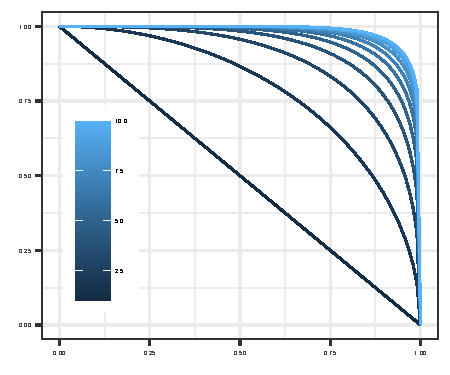
\includegraphics[width=0.10\textwidth]{images/p_sphere}
            ~
            \hspace{1cm}
            ~
            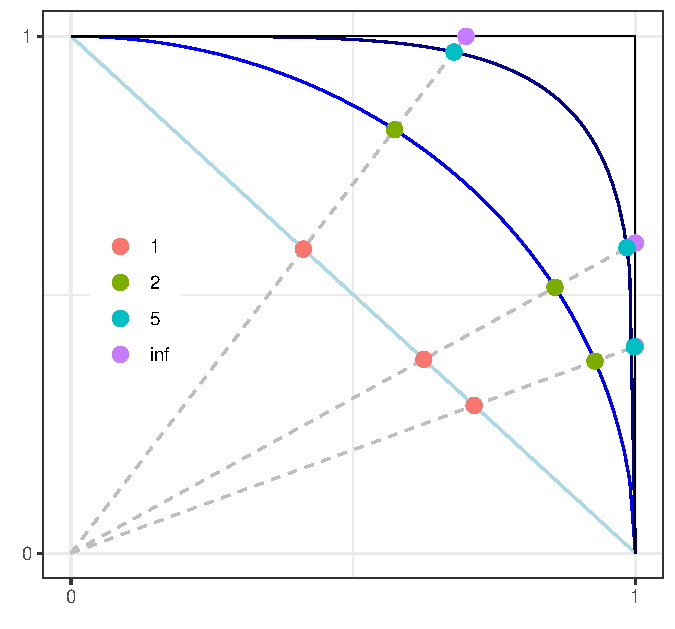
\includegraphics[width=0.10\textwidth]{images/p_project}
        \end{tikzfigure}
        \end{center}
        We recognize $\mathbb{S}_{\infty}^{d-1}$ as the positive orthant of the unit 
        hypersphere, under the $\mathcal{L}_{\infty}$ norm.  If we consider the 
        $\mathcal{L}_p$ norm, and then the $\mathbb{L}_{\infty}$ norm is expressed as the 
        limit of the $\mathcal{L}_p$ norm,
        \[
            \lVert \bm{s}\rVert_p = \left({\small\sum}_{\ell = 1}^d
                s_{\ell}^p\right)^{1/p},\;\;\;\;\;
            \lVert \bm{s}\rVert_{\infty} = 
            \lim\limits_{p\to\infty}\lVert \bm{s}\rVert_p = \bigvee_{\ell = 1}^d s_{\ell}.
        \]
        If we define $\mathbb{S}_{\infty}^{d-1}$ using this norm, then we consider it
        the limit of of an expanding series of manifolds $\mathbb{S}_p^{d-1}$, the
        positive orthant of the unit hypersphere under the $\mathcal{L}_p$ norm.  
        To establish a distribution on $\mathbb{S}_p^{d-1}$, we project a random 
        vector from $\mathbb{R}_+^d$ onto $\mathbb{S}_p^{d-1}$.  For 
        $\mathbb{x}\in\mathbb{R}_+^d$, let 
        $\bm{y} = \frac{\bm{x}}{\lVert\bm{x}\rVert_p} \in \mathbb{S}_p^{d-1}$.  Then, by letting 
        $y_d = \left(1 - \sum_{\ell = 1}^{d-1}y_{\ell}^p\right)^{\frac{1}{p}}$, the
        transformation
        \[T(x_1,\ldots,x_d) = \bigg(\lVert \bm{x}\rVert p, \frac{x_1}{\lVert \bm{x}\rVert_p}, 
                \ldots, \frac{x_{d-1}}{\lVert \bm{x}\rVert_p}\bigg)\]
        is invertible with
        \[T^{-1}(r,y_1,\ldots,y_{d-1}) = 
            \big(ry_1,\ldots,ry_{d-1},ry_d\big).\]
        The determinant of the Jacobian of this transformation takes the form
        \[r^{d-1}\left[y_d +
            {\tiny\sum}_{\ell = 1}^{d-1}y_{\ell}^py_d^{1 - p}\right].\]
        Integrating out $r$ will yield a distribution on $\mathbb{S}_p^{d-1}$.
        Note that for $p=\infty$, the transformation is no longer differentiable.  Thus, we 
        project $\bm{V}$ onto a large but finite $p$, and assess model fidelity on 
        $\mathbb{S}_{\infty}^{d-1}$
        }
   
\column{0.333}

\block{Projected Gamma Family \& DP Mixtures Thereof}
    {
    Given the form of the Jacobian, a natural distribution to consider in $\mathbb{R}_+^d$ is given by the product of 
    independent gamma distributions.  Let $\bm{X} \sim \prod_{\ell = 1}^d\text{Ga}(X_{\ell}\mid\alpha_{\ell},\beta_{\ell})$.  
    Using the transformation previously described, and treating $y_d = \left(1 - \sum_{\ell = 1}^{d-1}y_{\ell}^p\right)^{\frac{1}{p}}$, we have the joint density:
    \[
        f(r,\bm{y}\mid\bm{\alpha},\bm{\beta}) = \prod_{\ell = 1}^d \left[ \frac{\beta_{\ell}^{\alpha_{\ell}}}{\Gamma(\alpha_{\ell}}
            (ry_{\ell})^{\alpha_{\ell} - 1}\exp\lbrace-\beta_{\ell}ry_{\ell}\rbrace\right]\times 
            r^{d-1}\left[y_d +
            \sum_{\ell = 1}^{d-1}y_{\ell}^py_d^{1-p}\right].
    \]
    Integrating out $r$ yields the \emph{Projected Gamma} density,
    \[
    \text{PG}\left(\bm{y}\mid\bm{\alpha},\bm{\beta}\right) = \prod_{\ell = 1}^d
        \left[\frac{\beta_{\ell}^{\alpha_{\ell}}y_{\ell}^{\alpha_{\ell} - 1}}{\Gamma(\alpha_{\ell})}\right]
        \times \left[y_d +
            \sum_{\ell = 1}^{d-1}y_{\ell}^py_d^{1-p}\right]
        \times 
        \frac{\Gamma\left(\sum_{\ell = 1}^d\alpha_{\ell}\right)}{\left(\sum_{\ell = 1}^d
                \beta_{\ell}y_{\ell}\right)^{\sum_{\ell = 1}^d\alpha_{\ell}}}.
    \]
    For identifiability, we fix $\beta_1 := 1$. This creates a moderately flexible distribution on
    $\mathbb{S}_p^{d-1}$ for any finite $p$. The projected gamma family is simple to specify and
    has very tractable computational properties. Thus, we use it as a building block to model the 
    angular distribution.  To build a flexible family of distributions on $\mathbb{S}_p^{d-1}$, we build a Dirichlet process mixture of the form
    \[
    \bm{y}_i\mid (\bm{\alpha}_i,\bm{\beta}_i) \sim \text{PG}(y_i\mid\bm{\alpha}_i,\bm{\beta}_i), \;\;\;\;
    (\bm{\alpha}_i,\bm{\beta}_i) \mid G \sim G, \;\;\;\; G \sim \text{DP}(\eta,G_0).
    \]
    We consider 4 options:
    \begin{itemize}
        \item \emph{Projected Gamma} (PG) vs \emph{Projected Restricted Gamma} (PRG) kernel distribution
        \item \emph{Product of Gammas} (--G) vs \emph{Multivariate Lognormal} (--LN) centering distribution
    \end{itemize}
    }

\block{Scoring Criteria for Distributions on $\mathbb{S}_{\infty}^{d-1}$}
    {
    To assess and compare the fidelity we focus on \emph{energy score}.  This has a deceptively simple calculation: the score at observation $i$ is calculated as
    \[
        S(P,\bm{x}_i) = \text{E}_p\left[g(\bm{X}_i,\bm{x}_i\right] -
        \frac{1}{2}\text{E}_P\left[g(\bm{X}_i,\bm{X}_i^{\prime})\right],
    \]
    where $g$ is a negative definite kernel.  As the process we are trying to capture operates 
    on $\mathbb{S}_{\infty}^{d-1}$, ideally $g$ would be the geodesic distance in
    that space. Let \[\mathbb{C}_\ell^{d-1} = \lbrace
    \bm{x} : \bm{x} \in \mathbb{S}_{\infty}^{d-1}, x_{\ell} = 1\rbrace\] comprise the $\ell$th
    face of $\mathbb{S}_{\infty}^{d-1}$.  Geodesic distance in
    $\mathbb{S}_{\infty}^{d-1}$ is difficult, but for
    $\bm{a}\in\mathbb{C}_{\ell}^{d-1}$, $\bm{b}\in\mathbb{C}_{\jmath}^{d-1}$, 
    an upper bound can be established as
    \[
        g(\bm{a},\bm{b}) = \min\limits_{\bm{c}\in\mathbb{C}_{\jmath}^{d-1}\cap\mathbb{C}_{\ell}^{d-1}}\lbrace\lVert \bm{c} - \bm{a}\rVert_2 + \lVert \bm{b} - \bm{c}\rVert_2\rbrace.
    \]
    Under this construction, $g$ is a negative definite kernel, as it is the sum of two 
    negative definite kernels.  Calculating $g$ is made faster by rotating 
    $\bm{b}\in\mathbb{C}_{\jmath}^{d-1}$ into the same hyperplane as $\bm{a}\in\mathbb{C}_{\ell}^{d-1}$.
    % , 
    % by setting \[\bm{b}^{\prime} = \begin{cases}b_i &\text{ for }i\neq \jmath,\ell\\ 
    %     1 &\text{ for }i = \ell \\ 2 - b_{\ell} &\text{ for }i = j  \end{cases},\]
    % then $g(\bm{a},\bm{b}) = \lVert \bm{a} - \bm{b}^{\prime}\rVert_2$.
    }


    
\block{Future Work in Extreme Analysis}
    {
    \begin{itemize}[noitemsep]
        \item Novelty detection in extremes using the projected gamma representation:
            \begin{itemize}[noitemsep]
                \item Inference in $\mathbb{S}_{\infty}^{d-1}$ introduces new possibilities of applications.  We hope to create an unsupervised--learning method of spotting anomalies---data that is not \emph{normal}.
            \end{itemize}
        \item A variational approach to Dirichlet process mixtures of projected gammas:
        \begin{itemize}[noitemsep]
            \item The log-normal centering distribution, and MCMC techniques for sampling DP's in general induce a great deal of computational complexity.  Our goal is combating this problem through a variational approach.
        \end{itemize}
    \end{itemize}
    }
\column{0.333}

    \block{Results}{
    We conducted a simulation study to evaluate the performance of PG vs PRG, and ~--G vs ~--LN.
    
    \begin{tikzfigure}[Energy Score vs number of dimensions for recovering distribution of simulated data,\\for varying number of mixture components in generating distribution (lower is better).]
        \centering 
        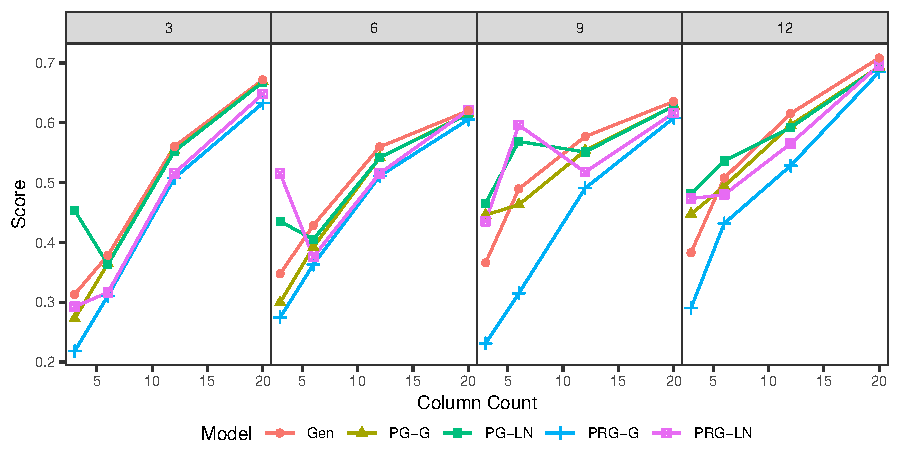
\includegraphics[width=0.25\textwidth,height=0.08\textwidth]{images/simulation_score_es}
    \end{tikzfigure}
    
    We see model fidelity was negatively affected by the additional 
    flexibility offered in the unrestricted model (PG vs PRG).
    Interesting to note here is that the Log-normal model offers slightly 
    worse performance as compared to the product of gammas. 
    
    \vspace{1cm}
    ~
    % Text and figure Inside the Block
    \begin{minipage}[c]{0.6\linewidth}
    
    We applied our models to two datasets for the \emph{integrated vapor transport} (IVT).
    This data captures the total amount of water vapor in the air in an atmospheric 
    column, over a cell grid along California's coast.  ERA--Interim has 9 columns; and 
    ERA5 has 43 columns.
    
    
    We see a slight reversal here, as compared to the simulation, where the log-normal 
    centering distribution is preferred for the high-dimensional data.  Again, the
    restricted model performs better than the unrestricted model.
    \end{minipage}%
    \begin{adjustbox}{valign=c}
    \begin{minipage}[t]{0.4\linewidth}
    \begin{tikzfigure}[Energy Score for fitted models against\\ IVT data (lower is better).]
        \centering
        \begin{tabular}{ccc}
        \toprule
        Model   & ERA--Interim  & ERA--5\\
        \midrule
        PRG--G  & {\bf 0.172}   & 0.751       \\
        PRG--LN & 0.173         & {\bf 0.714} \\
        PG--G   & 0.426         & 1.169       \\
        PG--LN  & 0.294         & 0.799       \\
        \bottomrule
        \end{tabular}
    \end{tikzfigure}
    \end{minipage}
    \end{adjustbox}
    }
\begin{subcolumns}
\subcolumn{0.5}
\block{Conditional Survival}{
    For a set of dimensions $\Omega\subset\lbrace1,\ldots,d\rbrace$, the conditional probability of survival for set $\Omega$ can be calculated as
    \[
    \medmath{
    \mathrm{Pr}\bigg[\cap_{\ell \in \Omega} Z_\ell > z_\ell \mid \cap_{\ell\not\in\Omega} Z_\ell > z_\ell\bigg]
    = \frac{\text{E}\left[\wedge_{k = 1}^d 1\wedge \frac{V_k}{z_k}\right]}{\text{E}\left[\wedge_{k \not\in\Omega}1\wedge\frac{V_k}{z_k}\right]}.
    }
    \]
    We see two such sets $\Omega$ here, holding all other dimensions at their respective fitted $90$th percentile.
    \begin{tikzfigure}[Conditional survival curves for 2 $\Omega$--sets given all others $\geq F^{-1}(0.9)$ (fitted), from ERA-Interim data with PRG--G model.  Left is original scale, right is standardized margins.]
    % \begin{wrapfigure}{L}{0.15\textwidth}
    \centering
    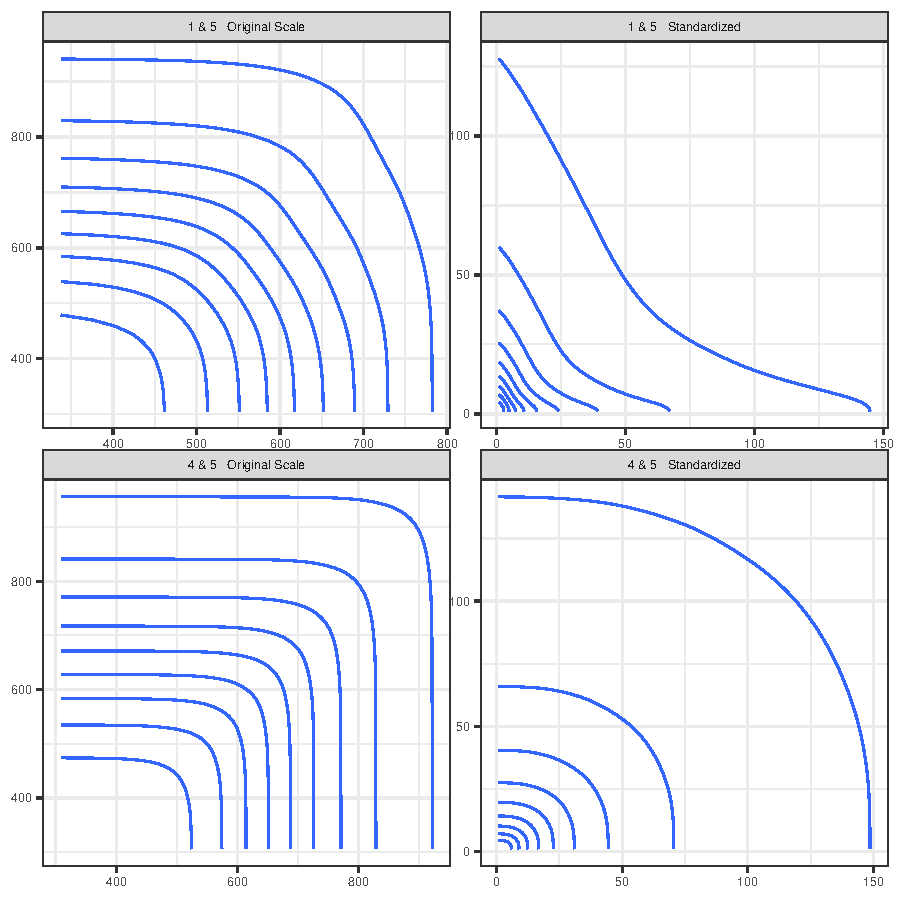
\includegraphics[width=0.12\textwidth]{./images/condsurv_2d}
    %     \caption{Conditional survival curves for 2 pairs of dimensions given all others $\geq F^{-1}(0.9)$ (fitted), from ERA-Interim data with PRG--G model.}
    % \end{wrapfigure}
    \end{tikzfigure}
}
\subcolumn{0.5}
\block{Extremal Dependence}{
    A measure to characterize the strength of dependence between two variables is the
    extremal dependence coefficient.  We establish the second equality
    as, by standardization, the marginal distribution of $Z_{\jmath}$ is the same as that of $Z_{\ell}$.
    \[
        \medmath{
        \begin{aligned}
        \chi_{\jmath\ell} &= \lim\limits_{u\uparrow 1}\text{Pr}\left[
        F_{\jmath}(Z_{\jmath}) > u \mid F_{\ell}(Z_{\ell}) > u\right]\\
        &= \text{E}\left[
        \frac{V_{\jmath}}{\text{E}[V_{\jmath}]}\bigwedge
        \frac{V_{\ell}}{\text{E}[V_{\ell}]}
        \right].
        \end{aligned}
        }
    \]
    Using a sample from the posterior predictive of a fitted PRG-G model on the IVT data, we compute this expectation numerically.
    
    \begin{tikzfigure}[Pairwise extremal dependence coefficients\\ for IVT data using PRG-G model.]
    \centering
    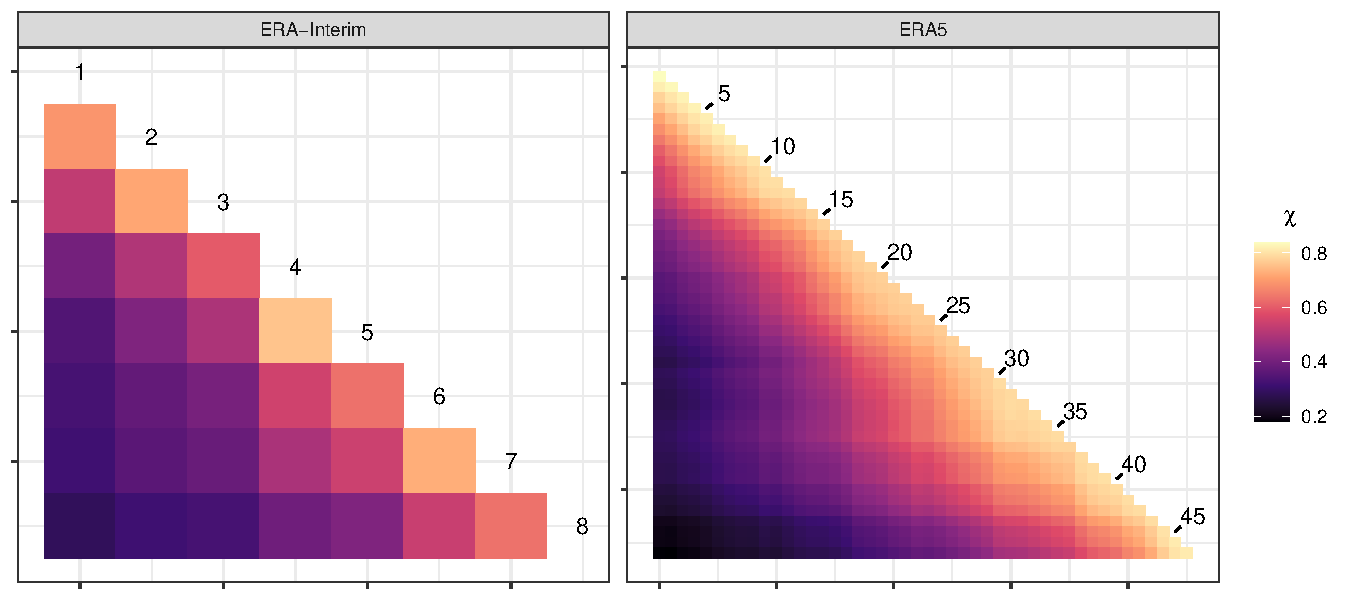
\includegraphics[width=0.95\linewidth]{./images/chi_ij_c}
    \end{tikzfigure}
    Effectively, using the model in this way, we are capturing the spatial dependence structure for extremes in the IVT.
    }
\end{subcolumns}
    
\end{columns}












% \block{Angular Distributions}{Here, \blindtext \vspace{4cm}}
%     \note[
%         targetoffsetx=-9cm, 
%         targetoffsety=-6.5cm, 
%         width=0.4\linewidth
%         ]
%         {e-mail \texttt{welcome@overleaf.com}}
% \begin{columns}
%     \column{0.5}
%     \block{A figure}
%     {
%         \begin{tikzfigure}
%             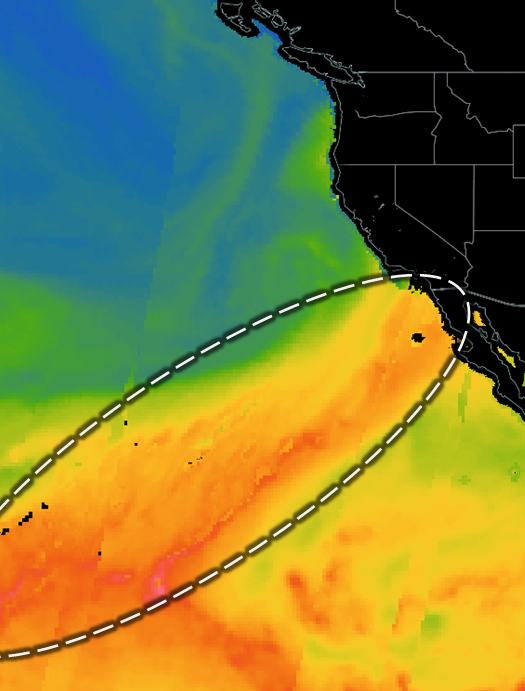
\includegraphics[width=0.4\textwidth]{images/ar}
%         \end{tikzfigure}
%     }
%     \column{0.5}
%     \block{Description of the figure}{\blindtext}
% \end{columns}

\end{document}
